\chapter{Introduction}\label{C:intro}
\section{The Problem} 
The objective of this project is to create a prototype application that will be used to support agile team retrospective meetings. This project is part of the aWall software project run by Dr. Craig Anslow and Professor Martin Kropp of FHNW in Switzerland.

The outcome of this project, is to build a software web system to help facilitate agile retrospective meetings using a large touch screen as an output for the software. Once this software has been built, an evaluation with users will occur to evaluate and improve on the software project. The current aWall project can be found here: \url{https://www.youtube.com/watch?v=fzCnjnpRiTI}

\begin{figure}[ht]
\centering
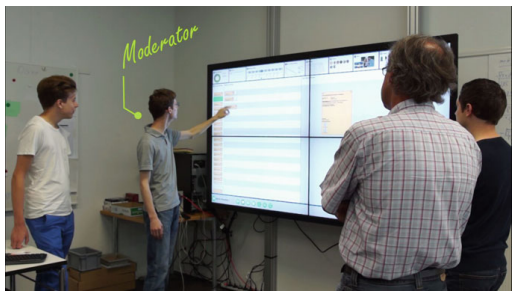
\includegraphics{aWall_introduction}
\caption{Project aWall - digital agile cardwall being used}
\end{figure}
\section{Overview of Research Project}
This project will be building off this current prototype but within its own project scope and no integration between the two codebases.

This software prototype is split into three different components:
\begin{itemize}
\item \textbf{Participant System:} The participant system is used for the participants to interact within the system, it is an application that will allow the participant to vote and make notes about the retrospective and directly interact with what is happening on the screen and within the retrospective. All the interactions from this system get send and stored within the database housed within the server. This system will be housed on a participants phone with a connection to the server through a socket.
\item \textbf{Screen System:} The screen system is an application that the moderator of the retrospective interacts with, it allows the moderator to display and manipulate the data passed from the server that the participants have given. This system will be used on the touch screen with a connection to the server through a socket.  
\item \textbf{Server:} The server houses all the data storage and manipulation for the overall software system. It also houses the socket system allowing for real-time updates between the participant and screen systems. It allows the storage of data for later use in later iterations of the projects lifecycle, e.g. a later agile retrospective. 
\end{itemize}

Within this prototype there will be different versions of agile retrospectives that the user can choose. The different retrospectives that were chosen were from my personal industry experience with agile and from academic literature \cite{AgileRetrospectivesEstherDerby} \cite{normanKeith}, these different types of retrospective are:
\begin{itemize}
\item The 3W's/Mad, Sad and Glad
\item Timeline
\item Brainstorm/Filtering
\item Short Subjects
\end{itemize}

Each of these retrospective methods will be able to be selected from the screen system within the software application when creating a retrospective session. To accompany each of these retrospective methods, there will also be short sections before and after the main method, it allows for the setting of the scene within the retrospective and to wrap up the retrospective also.

The methods that I have chosen for this are:  \cite{AgileRetrospectivesEstherDerby}
\begin{itemize}
\item \textbf{Setting the scene:} Check-in
\item \textbf{Wrapping-up:} +/- or Delta
\end{itemize}

Using each of these four methods, I will be able to evaluate the best retrospective method through testing with users.
